\documentclass[a4paper, twocolumn]{article}
\usepackage[landscape, a4paper, left=1cm, right=1cm, top=1cm, bottom=4cm]{geometry}
\usepackage[parfill]{parskip}
\usepackage{fancyhdr}
\usepackage{tikz}
\usepackage{xcolor}
\usepackage{listings}
\usepackage{amsmath}
\usepackage{titlesec}
\usepackage{tabularx}
\usepackage{graphicx}

% Colour definitions
\definecolor{SpecialBlue}{RGB}{0, 166, 214}

% Team Name
\newcommand{\teamname}{Crystal Math}
\newcommand{\teammembers}{Gabriëlle Zwaneveld, Sven Holtrop and Lucas Crijns}
% Useful commands
\renewcommand{\vec}{\overrightarrow}
\newcommand{\pageend}{\vfill\newpage}
\newcommand{\arrow}{$\rightarrow$ }
\newcommand{\ms}{\texttt}
\newcommand{\point}[4]{\draw[fill] (#1,#2) circle (1pt) node[#4] {#3}}
\newcommand{\note}{\textbf{Note: }}

% Fix Header
\setlength{\topmargin}{0cm}
\setlength{\headsep}{0cm}
\setlength{\columnsep}{1cm}
% Syntax Highlighting
\lstset{language=python}
\definecolor{mygreen}{rgb}{0,0.6,0}
\definecolor{mygray}{rgb}{0.5,0.5,0.5}
\definecolor{mymauve}{rgb}{0.58,0,0.82}

\lstset{ %
    backgroundcolor=\color{white},   % choose the background color; you must add \usepackage{color} or \usepackage{xcolor}
    basicstyle=\footnotesize\ttfamily,        % the size of the fonts that are used for the code
    breakatwhitespace=false,         % sets if automatic breaks should only happen at whitespace
    breaklines=true,                 % sets automatic line breaking
    captionpos=b,                    % sets the caption-position to bottom
    commentstyle=\color{mygreen},    % comment style
    deletekeywords={...},            % if you want to delete keywords from the given language
    escapeinside={\%*}{*)},          % if you want to add LaTeX within your code
    extendedchars=true,              % lets you use non-ASCII characters; for 8-bits encodings only, does not work with UTF-8
    frame=single,                    % adds a frame around the code
    keepspaces=true,                 % keeps spaces in text, useful for keeping indentation of code (possibly needs columns=flexible)
    keywordstyle=\color{blue},       % keyword style
    otherkeywords={*,...},           % if you want to add more keywords to the set
    %numbers=left,                    % where to put the line-numbers; possible values are (none, left, right)
    %numbersep=5pt,                   % how far the line-numbers are from the code
    %numberstyle=\tiny\color{mygray}, % the style that is used for the line-numbers
    rulecolor=\color{black},         % if not set, the frame-color may be changed on line-breaks within not-black text (e.g. comments (green here))
    showspaces=false,                % show spaces everywhere adding particular underscores; it overrides 'showstringspaces'
    showstringspaces=false,          % underline spaces within strings only
    showtabs=false,                  % show tabs within strings adding particular underscores
    %stepnumber=2,                    % the step between two line-numbers. If it's 1, each line will be numbered
    stringstyle=\color{mymauve},     % string literal style
    tabsize=2,                       % sets default tabsize to 2 spaces
    %title=\lstname                   % show the filename of files included with \lstinputlisting; also try caption instead of title
}



% Pagestyle
\renewcommand{\familydefault}{\sfdefault}
\pagestyle{fancy}
\newcommand{\mkfoot}{
	\begin{tikzpicture}[remember picture,overlay]
		\node[yshift=0] at (current page.south west) {
			\begin{tikzpicture}[remember picture,overlay]
				\fill [SpecialBlue] (0cm, 0cm) rectangle (\paperwidth, 1.5cm);
			\end{tikzpicture}
		};
		\node[yshift=-2cm] at (current page.north west) {
			\begin{tikzpicture}[remember picture, overlay]
				\fill [SpecialBlue] (0cm, 0cm) rectangle (\paperwidth, 2cm);
				\node at (\paperwidth - 2.5cm, 0.7cm) {
\includegraphics[height=3cm]{logo.eps}};
			\end{tikzpicture}
		};
	\end{tikzpicture}
}
\fancyhead{\mkfoot}
\fancyfoot{}
\fancyfoot[L]{\color{white} \large \textbf{\teamname} Cheatsheet}
\fancyfoot[R]{\color{white} \teammembers \hspace{1.3em} \large \textbf\thepage}
\renewcommand{\headrulewidth}{0cm}
\renewcommand{\headrulewidth}{0cm}

\titlespacing*{\section}{0pt}{1.0pt plus 0.5pt minus .2pt}{0.8pt plus .2pt}
\titlespacing*{\subsection}{0pt}{1.0pt plus 0.5pt minus .2pt}{0.8pt plus .2pt}


\begin{document}

% Title page
\begin{titlepage}
	\centering
	~\\
	\vspace{20px}
	\resizebox{700px}{!}{\Huge Team Contest Reference}
	\\ \vspace{40px}
	\resizebox{400px}{!}{\Huge \textcolor{SpecialBlue}{\textbf{\teamname}}}
	\\ \vspace{20px}
	\resizebox{500px}{!}{\LARGE \teammembers}
	
\includegraphics[width=300px]{logo_rgb.eps}
\end{titlepage}

\section{Modules}
\subsection{Python}
\begin{itemize}
	\item Priority queue \arrow \ms{heapq}
	\item Python base switching \arrow \ms{int(x, base=b)}
	\item Deque \arrow \ms{collections.deque}
\end{itemize}
\subsection{C++}
\begin{itemize}
	\item \ms{std::pair<T,G>, std::make\_pair} \arrow \ms{\#include <utility>}
	\item \ms{std::vector<T>} \arrow \ms{\#include <vector>}
	\item \ms{std::queue<T>} (Priority queue) \arrow \ms{\#include <queue>}
\end{itemize}

\section{Mathematics}
\subsection*{Formulas for Geometric Shapes}
\vspace{-1em}
\begin{align*}
\text{oppervlakte cirkel}   &: \pi r^2 \\
\text{omtrek cirkel}        &: \pi d \\
\text{oppervlakte ellips}   &: \pi a b \\
\text{oppervlakte kegel}    &: \pi r^2 + \pi r \sqrt{r^2 h^2} \\
\text{inhoud kegel}         &: \frac{1}{3}\pi r^2 h \\
\text{oppervlakte bol}      &: 4 \pi r^2 \\
\text{inhoud bol}           &: \frac{4}{3} \pi r^3 \\
\text{oppervlakte cillinder}&: 2\pi rh + 2\pi r^2 \\
\text{inhoud cilinder}      &: \pi r^2 h\\
\end{align*}

\subsection{Trapezion}
oppvervlakte trapezium: $\frac{a+b}{2}h$\\
Als de evenwijdige zijden $a,b$ verschillende lengtes hebben, dan is h:
\begin{align*}
h = \frac{\sqrt{(-a+b+c+d)(a-b+c+d)(a-b+c-d)(a-b-c+d)}}{2|b-a|}
\end{align*}
De lengtes van de diagonalen als $b>a$ de evenwijdige zijden zijn
\begin{align*}
p &= \sqrt{\frac{ab^2-a^2b-ac^2+bd^2}{b-a}}\\
q &= \sqrt{\frac{ab^2-a^2b-ad^2+bc^2}{b-a}}
\end{align*}

\subsection{Oppervlakte formules}
Formule van Heron:\\
$$s = \frac{a+b+c}{2}$$
$$\sqrt{s(s-a)(s-b)(s-c)}$$

Bretschneider's formule:\\
$$s = \frac{a+b+c+d}{2}$$
$$\sqrt{(s-a)(s-b)(s-c)(s-d)-abcd cos^2\left(\frac{\alpha+\gamma}{2}\right)}$$

\subsection*{More Formulas}
\begin{align*}
\text{least common multiple} &: \text{lcm}(m, n) = \frac{|m \cdot
	n|}{\text{gcd(m, n)}} \\
\text{Catalan number} &: C_n = \frac{1}{n+1}{2n \choose n} =
\frac{(2n)!}{(n+1)!n!} = \prod^n_{k=2}\frac{n+k}{k} \\
\text{Catalan numbers} &: C = \{1, 1, 2, 5, 14, 42, 132, 429, 1430, 4862,
16796\}
\end{align*}
\vspace{-1em}
\subsection*{Fibonacci Numbers}\vspace*{-1em}
\begin{align*}
1,1,2,3,5,8,13,21,34,55,89, 144, 233, 377, 610, 987, 1597, 2584
\end{align*}
\begin{itemize}
	\item  When we take a pairs of large consecutive Fibonacci numbers, we can
	approximate the golden ratio by dividing them.
	\item The sum of any ten consecutive Fibonacci numbers is divisible by 11.
	\item Two consecutive Fibonacci numbers are co-prime.
	\item The Fibonacci numbers in the composite-number (i.e. non-prime)
	positions are also composite numbers.
\end{itemize}
\subsection{Vectoren}
\textbf{Cross product}
\begin{align*}
a \times b &= \begin{bmatrix} a_x \\ a_b \\ a_z \end{bmatrix}
\times \begin{bmatrix} b_x \\ b_y \\ b_z \end{bmatrix} =
\begin{bmatrix} a_yb_z - a_zb_y \\ a_zb_x - a_xb_z \\ 
a_xb_y - a_yb_x \end{bmatrix}
\end{align*}
De projectie van een vector x op een andere vector y is:
$$\frac{\langle x,y \rangle}{\langle y,y \rangle} y$$
Het verschil van x en zijn projectie op y, staat loodrecht op y.\\
Twee vectoren x en y zijn loodrecht dan en slechts dan als $\langle x,y \rangle = 0$.\\

Projectie van een vector x op een vlak V. Bereken een normaal vector van V, bereken projectie p' van x op n. De projectie van x op V is dan x-p'.\\


\subsection*{Links of rechts ombuigen}\vspace{-0.5em}
\begin{minipage}{0.45\linewidth}
	\begin{tikzpicture}
	\draw[->, >=latex] (0mm, 0mm) node[left] {A} -- (15mm, 10mm) node[above left] {B};
	\draw[->, >=latex] (15mm, 10mm) -- (40mm, 20mm) node[above] {C};
	\end{tikzpicture}
\end{minipage}
\begin{minipage}{0.25\linewidth}
	\begin{align*}
	\vec{AB} &= \begin{bmatrix} p \\ q \end{bmatrix} \\
	\vec{n} &= \begin{bmatrix} q \\ -p \end{bmatrix} \\
	\end{align*}
\end{minipage}%
\begin{minipage}{0.25\linewidth}
	\begin{align*}
	\vec{n} &\cdot \vec{BC} < 0 \Rightarrow \text{linksaf} \\
	\vec{n} &\cdot \vec{BC} > 0 \Rightarrow \text{rechtsaf}
	\end{align*}
\end{minipage}
\subsection*{Punt in concaaf/convex polygon test}
Tel het aantal doorsnijdingen van polygon met lijn $P$ naar oneindig. Als het
aantal \\ doorsnijdingen oneven is, dan $P \in ABCDE$. \\
\begin{minipage}{.45\linewidth}
	\begin{align*}
	\alpha &= \angle APB + ... + \angle DPE + \angle EPA \\
	\alpha &= 0 \Rightarrow P \notin ABCDE \\
	\alpha &= 2\pi \Rightarrow P \in ABCDE
	\end{align*}
\end{minipage}\hfill%
\begin{minipage}{.5\linewidth}
	\centering
	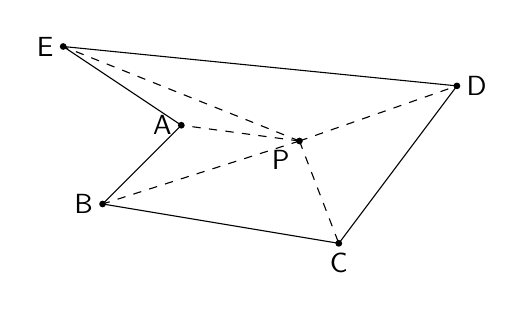
\begin{tikzpicture}
	\point{20mm}{0mm}{A}{left};
	\point{10mm}{-10mm}{B}{left};
	\point{40mm}{-15mm}{C}{below};
	\point{55mm}{5mm}{D}{right};
	\point{5mm}{10mm}{E}{left};
	\point{35mm}{-2mm}{P}{below left};
	\draw (20mm,0mm) -- (10mm,-10mm) -- (40mm, -15mm) -- (55mm, 5mm) --
	(5mm,10mm) -- (20mm, 0mm);
	\draw[dashed] (35mm, -2mm) -- (20mm, 0mm);
	\draw[dashed] (35mm, -2mm) -- (10mm, -10mm);
	\draw[dashed] (35mm, -2mm) -- (40mm, -15mm);
	\draw[dashed] (35mm, -2mm) -- (55mm, 5mm);
	\draw[dashed] (35mm, -2mm) -- (5mm, 10mm);
	\end{tikzpicture}
\end{minipage}

\vspace{-1.8em}
\subsection*{Centroid of polygon} \vspace{-0.3em}
The centroid or geometric center of a plane figure is the arithmetic mean
("average") position of all the points in the shape. Informally, it is the point
at which an infinitesimally thin cutout of the shape could be perfectly balanced
on the tip of a pin.
\vspace{-0.5em}
\begin{align*}
C_x &= \frac{1}{6A}\sum_{i=0}^{n-1}(x_i+x_{i+1})(x_iy_{i+1}-x_{i+1}y_i) \\
C_y &= \frac{1}{6A}\sum_{i=0}^{n-1}(y_i+y_{i+1})(x_iy_{i+1}-x_{i+1}y_i) \\
A   &= \frac{1}{2}\sum_{i=1}^{n-1}(x_iy_{i+1}-x_{i+1}y_i)
\end{align*}
\subsection*{Point to line distance}
\begin{equation*}
	d(ax+by+c=0, (x_0, y_0)) = \frac{|ax_0+by_0+c|}{\sqrt{a^2+b^2}}
\end{equation*}
\subsection*{Number theory}
$d(n)$ is het aantal positieve delers van een positief geheel getal $n$, met 1 en $n$ inbegrepen.
\begin{align*}
	d(1) + d(2) + \ldots + d(n) &= \lfloor \frac{n}{1} \rfloor + \lfloor \frac{n}{2} \rfloor + \ldots + \lfloor \frac{n}{n} \rfloor
\end{align*}

Aantal factoren van een priemgetal $a$ in $n!$ is:
\begin{align*}
	\lfloor \frac{n}{a} \rfloor + \rfloor \frac{n}{a^2} \rfloor + \ldots
\end{align*}
Kleine stelling van Fermat, $p$ priem en $a>0$:
\begin{align*}
	a^p \equiv a \mod p
\end{align*}
Als $a$ en $p$ copriem zijn:
\begin{align*}
	a^{p-1} \equiv 1 \mod p
\end{align*}
\subsection*{Series and sums}
Geometric series with $r$:
\begin{align*}
	a + ar^2 + \ldots + ar^{n-1} &= \sum^{n-1}_{k=0} ar^{k} = a\left(\frac{1-r^n}{1-r}\right) \\
	\lim_{n\rightarrow \infty} S &= \frac{a}{1-r} \quad \forall |r| < 1
\end{align*}
\begin{align*}
    \sum_{i=1}^n i &= \frac{n(n+1)}{2} \\
    \sum_{i=1}^n i^2 &= \frac{n(n+1)(2n+1)}{6} \\
    \sum_{i=1}^n i^3 &= \frac{n^2(n+1)^2}{4}
\end{align*}
\subsection{Lagrange polynomials}
Given a set of (k+1) data points $(x_0,y_0),(x_1,y_1), \ldots (x_k,y_k)$ where no two $x_j$ are the same. Find a polynomial of degree $k$ that has all $(k+1)$ points
\begin{align*}
L(x) &= \sum_{j=0}^k y_jl_j(x) \\
l_j(x) &= \prod_{0 \leq m \leq k, m \neq j} \frac{x-x_m}{x_j-x_m} \\
\end{align*}

\subsection*{Graphs}
For a connected planar graph, the number of vertices $V$, edges $E$ and planar faces $F$ obeys: $V-E+f=2$ (this includes the outer face).

\section{Algorithms}

%PLACEHOLDER%

\end{document}
